\documentclass{report}
\usepackage[spanish]{babel}
\usepackage[utf8]{inputenc}
\usepackage{graphicx, longtable, float, titlesec, hyperref}

\hypersetup{
    hidelinks = true
}

\titleformat{\chapter}[display]
  {\normalfont\bfseries}{}{0pt}{\Huge}

\begin{document}
    \begin{titlepage}
        \centering
        
\includegraphics[width=0.6\textwidth]{./img/miscelanio/logo.jpg}\\
        \vspace{1cm}
        \LARGE Sistemas de Gestión de Seguridad de Sistemas de Información\\
        \vspace{0.5cm}
        \Large Ingeniería Informática de Gestión y Sistemas de Información\\
        \vspace{3cm}
        \Huge Sistema Web\\
        \vspace{2.5cm}
        \Large Autores:\\
        \vspace{0.2cm}
        \large Xabier Gabiña\\
        \large Ainhize Martinez\\
        \large Marcos Martín\\
        \vfill
        \today
    \end{titlepage}
    \tableofcontents
    \chapter{Introduccion}
    \chapter{Primera auditoria}
        La idea de esta auditoria es la de encontrar los fallos de seguridad que tiene nuestro sistema web para en el posterior capitulo de este documento comentarlos y solucionarlos.\\

        \section{ZAP}
        Para empezar con la primera auditoria ejecutaremos el proxy ZAP como se nos ha propuesto en clase.
        Al ejecutarla en nuestra pagina web nos encontramos con el siguiente listado de errores:
        \begin{figure}[H]
            \centering
            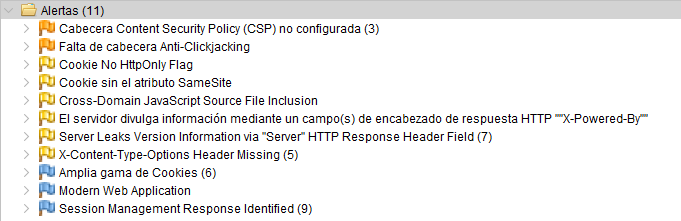
\includegraphics[width=\textwidth]{./img/audit1/zap1.png}
            \caption{Listado de errores de la primera auditoria}
        \end{figure}
        Como podemos ver en la imagen, tenemos un total de 11 errores, los cuales iremos comentando uno a uno en los siguientes apartados y solucionando.

        \section{sqlmap}

        \section{Metaexploit}
    \chapter{Vulnerabilidades}
        \section{Rotura de control de acceso}
            La rotura de control de acceso es una vulnerabilidad que permite a un atacante acceder a recursos restringidos o privilegiados, ya sea por un error en la implementación de la autenticación y autorización o por un error en la lógica de control de acceso.
            Dentro de nuestro sistema tenemos varios fallos de rotura de control y ahora hablaremos de ellas y de como las hemos solucionado.
            \subsection{Control de acceso}
                \subsubsection{Descripción}
                    En nuestro sistema, un usuario puede modificar sus datos personales, pero también puede modificar los datos de otros usuarios. 
                    Esto es un fallo de rotura de control de acceso ya que un usuario no debería poder modificar los datos de otro usuario.
                \subsubsection{PoC}
                    Pongamos en el ejemplo que tenemos dos usuarios, Admin y Xabier con sus repectivas IDs
                    \begin{figure}[H]
                        \centering
                        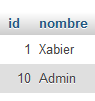
\includegraphics[width=0.2\textwidth]{./img/vulnerabilidades/3.1.1.1.png}
                        \caption{Datos de Usuarios}
                    \end{figure}
                    Si desde inspeccionar elementos hacemos click sobre el boton 'Perfil' este nos mostrara el link el cual se ve asi:
                    \begin{figure}[H]
                        \centering
                        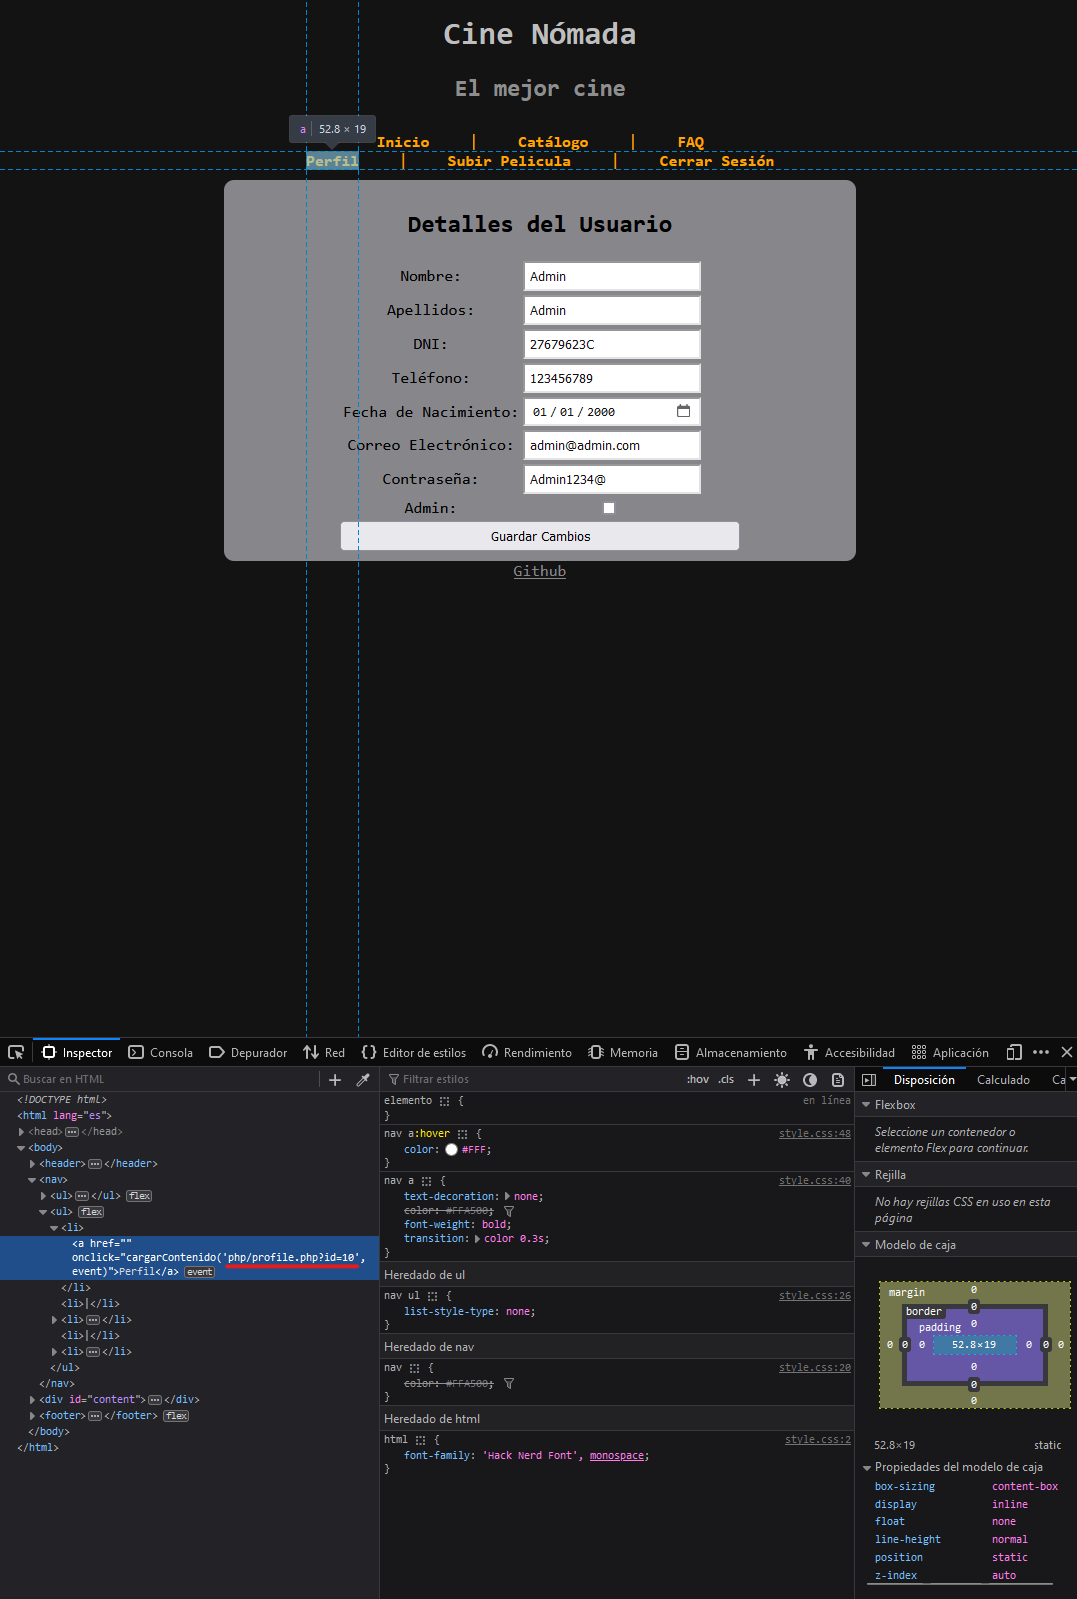
\includegraphics[width=0.8\textwidth]{./img/vulnerabilidades/3.1.1.2.png}
                        \caption{Perfil de Admin}
                    \end{figure}
                    Si alteramos el valor de ?id=X por en este caso la id de Xabier (La ID 1) podemos acceder a sus datos
                    \begin{figure}[H]
                        \centering
                        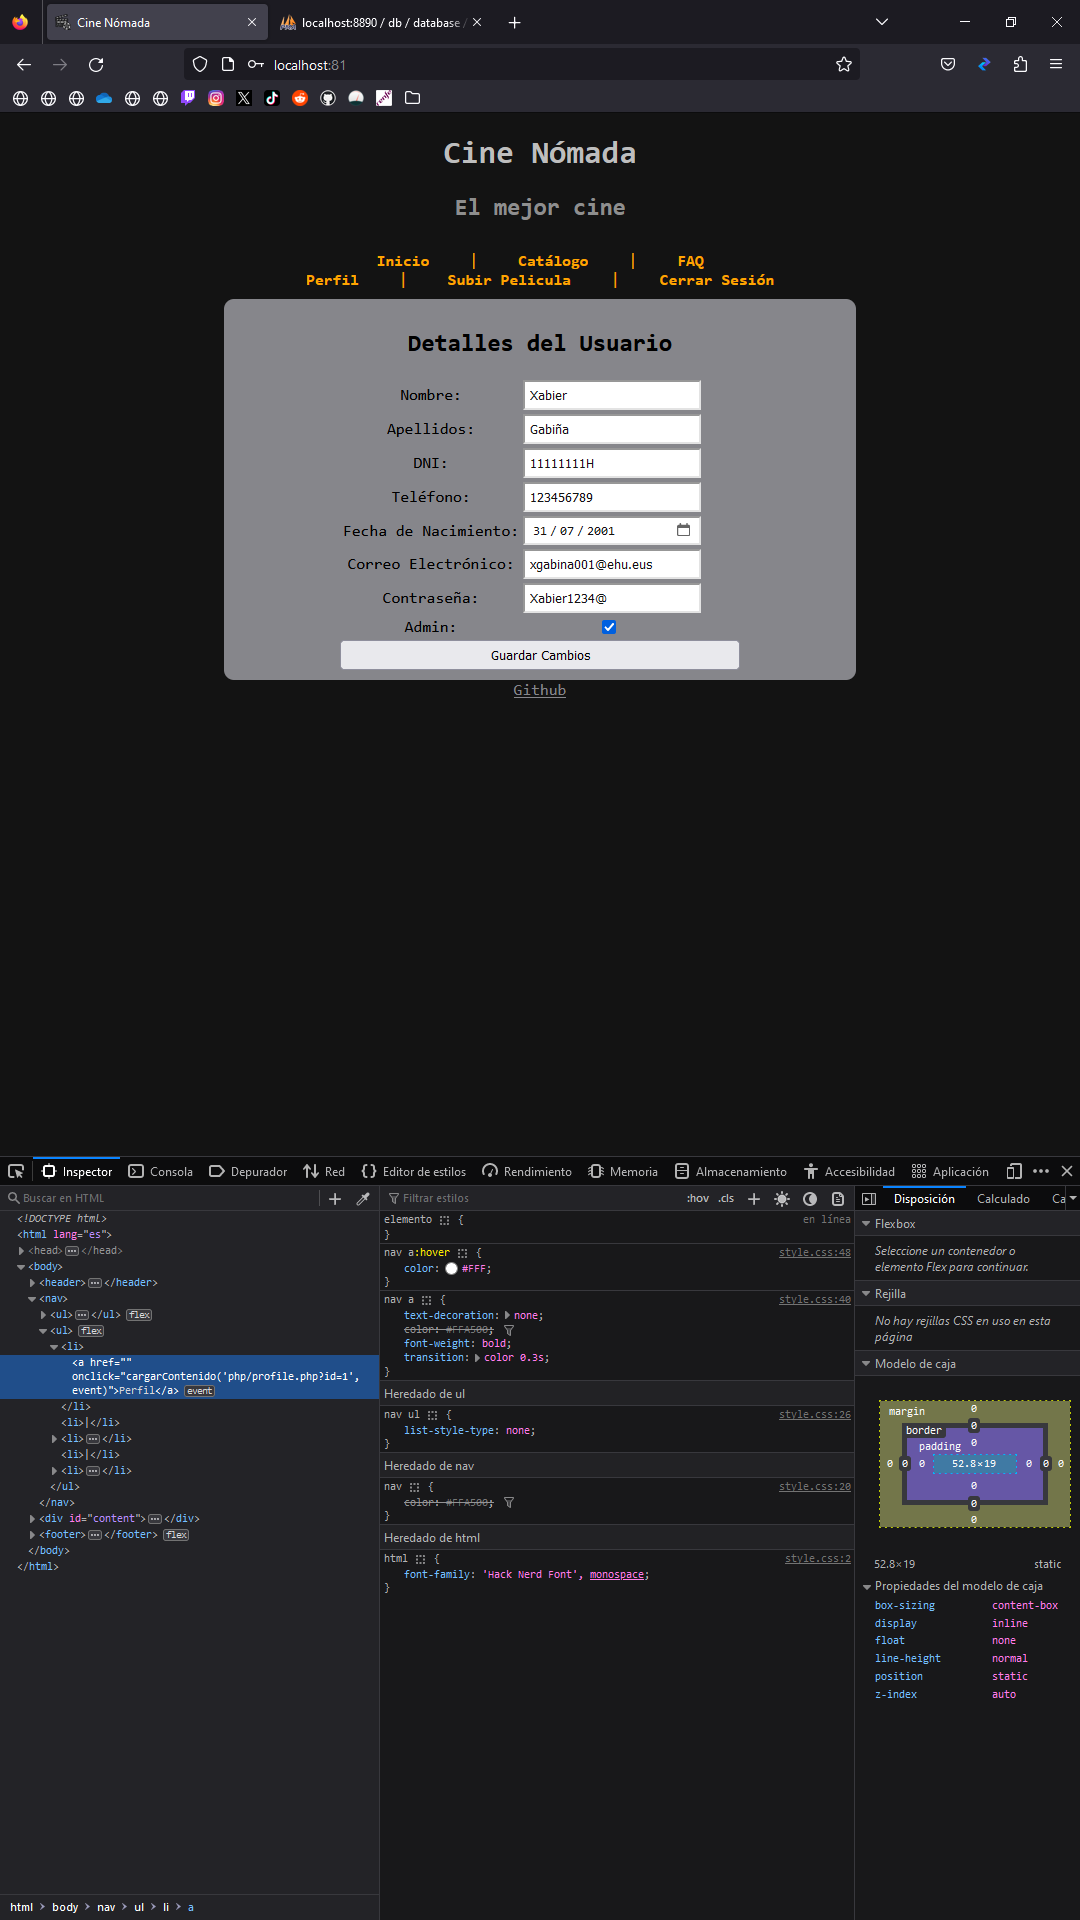
\includegraphics[width=\textwidth]{./img/vulnerabilidades/3.1.1.3.png}
                        \caption{Perfil de Xabier}
                    \end{figure}
                \subsubsection{Solución}
                    Para solucionar este problema, hemos añadido una comprobación en el código que comprueba que el usuario que está intentando modificar los datos es el mismo que el usuario que está logueado en el sistema.
                    \begin{figure}[H]
                        \centering
                        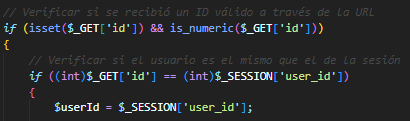
\includegraphics[width=\textwidth]{./img/vulnerabilidades/3.1.1.4.png}
                        \caption{Comprobación de usuario}
                    \end{figure}
                    Esta misma error tambien ha sido corregido en el catalogo.
            \subsection{Configuracion erronea de las Cookies}
                \subsubsection{Descripción}
                    En nuestro sistema, las cookies no tienen la configuración segura, lo que permite que un atacante pueda obtener información sensible de los usuarios.
                \subsubsection{Solución}
                    Para solucionar este problema, hemos añadido la configuración segura a las cookies.
                    \begin{figure}[H]
                        \centering
                        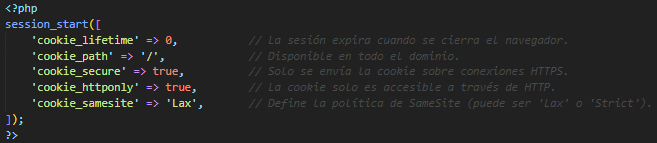
\includegraphics[width=\textwidth]{./img/vulnerabilidades/3.1.2.1.png}
                        \caption{Configuración de las cookies}
                    \end{figure}
        
        \clearpage
        \section{Fallos criptográficos}
            \subsection{Forzar HTTPS}
                \subsubsection{Descripción}
                    En nuestro sistema, no se fuerza el uso de HTTPS, lo que permite que un atacante pueda interceptar el trafico de la pagina y obtener información sensible de los usuarios.
                \subsubsection{Solución}
                    Para solucionar este problema configuraremos nuestro servidor para que cifre y rediriga todo el trafico a HTTPS.
            \subsection{Deshabilitar el almacenamiento en cache}
                \subsubsection{Descripción}
                    En nuestro sistema, no se deshabilita el almacenamiento en cache, lo que permite que un atacante pueda obtener información sensible de los usuarios.
                \subsubsection{Solución}
                    Para solucionar este problema crearemos una cabecera "Cache-Control" con el valor "no-store" para que el navegador no almacene en cache la pagina.
                    \begin{figure}[H]
                        \centering
                        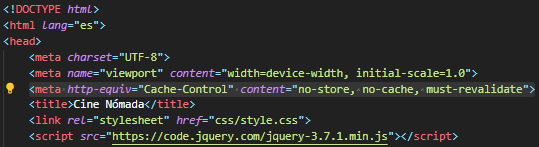
\includegraphics[width=\textwidth]{./img/vulnerabilidades/3.2.2.1.png}
                        \caption{Cabecera Cache-Control}
                    \end{figure}
            \subsection{Almacenamiento de contraseñas}
                \subsubsection{Descripción}
                    En nuestro sistema, no se almacenan las contraseñas de los usuarios de forma segura, lo que permite que un atacante pueda obtener las contraseñas de los usuarios.
                \subsubsection{PoC}
                    Si un atacante consigue acceso a la base de datos, puede obtener las contraseñas de los usuarios en texto plano.
                    \begin{figure}[H]
                        \centering
                        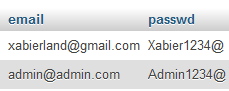
\includegraphics[width=\textwidth]{./img/vulnerabilidades/3.2.3.1.png}
                        \caption{Contraseñas en texto plano}
                    \end{figure}
                \subsubsection{Solución}
                    Para solucionar este problema, hemos añadido una función que cifra las contraseñas de los usuarios antes de almacenarlas en la base de datos.
                    \begin{figure}[H]
                        \centering
                        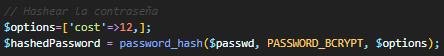
\includegraphics[width=\textwidth]{./img/vulnerabilidades/3.2.3.2.png}
                        \caption{Contraseñas cifradas}
                    \end{figure}
        \clearpage
        \section{Inyección}
            \subsection{Procesado de consultar SQL}
                \subsubsection{Descripción}
                    En nuestro sistema, no se procesan correctamente las consultas SQL, lo que permite que un atacante pueda obtener información sensible de los usuarios.
                \subsubsection{PoC}
                \subsubsection{Solución}
                    Para solucionar este problema, hemos modificado el codigo que procesa las consultas SQL para que no se puedan inyectar consultas SQL.
                    \begin{figure}[H]
                        \centering
                        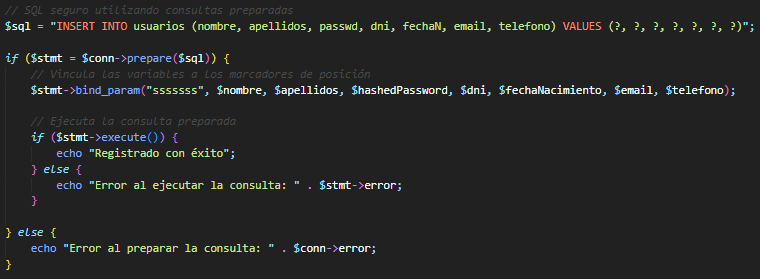
\includegraphics[width=\textwidth]{./img/vulnerabilidades/3.3.1.1.png}
                        \caption{Parametrizar consulta SQL}
                    \end{figure}
        \clearpage
        \section{Diseño inseguro}
            \subsection{Auditorias de seguridad}
            \subsection{Reutilizacion de codigos seguros}
        \clearpage
        \section{Configuración de seguridad insuficiente}
            \subsection{Entornos de desarrollo}
            \subsection{Plataforma minima}
            \subsection{Despliegue seguro}
            \subsection{Cabeceras CSP}
                \subsubsection{Descripción}
                    Estableces una CSP en un sitio web sirve para mejorar la seguridad de tu aplicación web y reducir el riesgo de ataques de seguridad. 
                    Una CSP especifica las fuentes de las que se pueden cargar recursos (como scripts, estilos, imágenes, etc.) en una página web.
                \subsubsection{Solución}
                    Para solucionar este problema, hemos añadido una cabecera "Content-Security-Policy" con los siguientes valores:
                    
                    Tambien hemos añadido X-Frame-Options para evitar ataques de clickjacking.
        \clearpage
        \section{Componentes vulnerables y obsoletos}
            \subsection{Control de versiones de los componentes}
                \subsubsection{Descripción}
                    En nuestro sistema no se utilizan las ultimas versiones de todos los componentes lo que puede resultar en una brecha de seguridad.
                \subsubsection{Solución}
                    Para solucionar este problema, hemos actualizado todos los componentes a sus ultimas versiones.
                    \begin{itemize}
                        \item PHP 7.2.2 → 8.2
                        \item MariaDB 10.8.2 → 11.1.2
                        \item phpMyAdmin ya estaba en la ultima version.
                        \item jQuery 3.6.0 → 3.7.1
                    \end{itemize}
        \clearpage
        \section{Fallos de identificación y autenticación}
            \subsection{Evitar ataques automatizados}
            \subsection{Contraseñas debiles o por defecto}
            \subsection{Autenticacion de dos factores}
            \subsection{Invalidacion de sesiones}
        \clearpage
        \section{Fallos en la integridad de datos y software}
            \subsection{Firmas digitales}
            \subsection{Bibliotecas y dependencias confiables}
            \subsection{Uso de herramientas de analisis}
        \clearpage
        \section{Fallos en la monitorizacion de la seguridad}
            \subsection{Implementacion de un log}
        \clearpage
        \section{Falsificacion de Solicitud del Lado del Servidor (SSRF)}
            \subsection{Control del trafico}
            \subsection{Asegurar el codigo}
        \clearpage
        \section{Problemas de calidad de codigo}
            \subsection{Revision de calidad del codigo}
        \clearpage
        \section{Problemas de denegacion de servicios}
            \subsection{Pruebas de rendimiento}
    \chapter{Segunda auditoria}
    \chapter{Conclusiones}
    \chapter{Bibliografia}
        \begin{itemize}
            \item OWASP. (2021). Informe de Vulnerabilidades. OWASP. \url{https://owasp.org/www-project-top-ten/}
            \item GPT-3.5. (2023). Respuestas a preguntas varias. OpenAI. \url{https://www.openai.com/}
            \item GitHub Copilot. (2022). Autocompletado. GitHub. \url{https://github.com/features/copilot}
        \end{itemize}
\end{document}